\section{Introduction}

The crucial question of the artificial intelligence is understanding what natural intelligence is. Unfortunately there are no aliens so far who would be able to demonstrate non-human intelligence, and examples on Earth lack certain substance. Rosalind Picard in her article indicated: "There may exist a kind of alien intelligent living system, something we’ve never encountered, which achieves its  intelligence without having anything like emotion. Although humans are the most marvellous example of intelligence we have, and we wish to build systems that are natural for humans to understand, these reasons for building human-like systems should not limit us to thinking only of human abilities." \cite{affectivecomputingchallanges}

There are several domains that still remain unclear: creativity, intuition, insight and consciousness that prevent us from answering the question: "How David Lynch could create Mulholland Drive or Picasso could create Guernica?". One aspect of modern AI is affective computation that become more and more important it is based on several domains: psychology: \cite{natureofemotions, appraisal_determinants_of_emotions, appraisal_considered_as_a_process, putting_appraisal_in_context, sex_differencies}, neuroscience: \cite{emotionsbraintorobot, parsingreward, neuromodulatory, cubeofemotions, natureofemotions, putting_appraisal_in_context, anatomic}, computer science: \cite{intelligent_machinery, emotionandsociable, senticcomputing, hourglass, affectivemodelofinterplay, affectivecomputing, dont_worry_be_happy, hourglass, senticcomputing, parsingreward, emotionsbraintorobot, motivationalrewardframework, roleofemotions, computationalmodelsemotionscognition}.

Turing stated in his report ``Intelligent Machinery'' \cite{intelligent_machinery} that idea of intelligent machines "cannot be wholly ignored, because the idea of 'intelligence' is itself emotional rather than mathematical".
There is an interconnection between emotions and rational thought. Marvin Minsky in his book "The emotion machine" \cite{emotionmachine} proposed that emotions are inseparable from thinking: "Emotional thinking: A flash of impatience or anger can cut through what seems like a hopelessly tangled knot. Each such 'emotional way to think' is a different way to deal with things, and some can increase your persistence or courage, while others can help you simplify things. In any case, after each such change, you may still want to pursue some similar goals, but now you'll see them from new points of view — because each switch to a new Way to Think may initiate a large-scale cascade. Then, depending on how long those changes persist, you (or your friends) might recognize this as a change in your emotional state".

Antonio R. Damasio in his work ``Emotion in the perspective of an integrated nervous system'' \cite{emotionInPerspectiveOfIntegratedNervousSystem} emphasized the effect of emotions: ``The ultimate results of emotion are of two kinds. First there are behaviors — the expressing of joy, or anger, or disgust — which affect interactions with other living creatures. Second, there are experiences of emotional states, that is feelings, which affect the ongoing thinking of the subject and by so doing can alter future thinking, future planning and future behavior.''

The other interesting point of view was represented by Ziemke and Lowe \cite{on_role_of_emotion, emotionsbraintorobot} ``Do robots need emotions? A pragmatic answer would be that robots, as currently conceived and constructed, simply do not have any needs (of their own) in the first place—and thus of course neither need emotions, nor energy, nor sensors, actuators, etc. A more relevant question then may be whether or not we, the human designers and users of robots, need or want robots to have or at least express emotions.''

Good review of computational models of emotions was presented by Jonathan Gratch and Stacy Marsella \cite{evaluatingcomutationalmodel, computationalmodelsemotion}. We have found several more computational emotions models created \cite{computationalmodelsemotion, computationalmodelsemotionscognition, evaluatingcomutationalmodel, threelevel}.

This work is dedicated to modeling of mapping of impacts of monoamine neuromodulators on human brain on a computational processes of modern computers. We propose the approach to correlate biochemical influence of monoamines: dopamine, serotonin, noradrenaline, involved in affective processing \footnote{In this article we use affects and emotions as notions with the same or close meaning, usually affects are used in sections dedicated to ``Theory of affects'' \cite{tomkins1, tomkins2, tomkins3} or derivatives \cite{cubeofemotions}, emotions on the other hand are used in context of Plutchik ``Wheel of emotions'' \cite{natureofemotions}.} of cortical, limbic and other subsystems of human brain with a computational processes: computational power, memory distribution, learning, storage, decision making that take place in computational systems. It could be considered as a base of affective computation framework and we hope could be used in several domains like:

\begin{enumerate}
 \item  Advertisement
 \item  Emotional behavior simulations
 \item  Robotics
 \item  Intellectual assistants
 \item  Estimating human behaviour
 \item  Nursing
\end{enumerate}

\section{Bases}

Starting from the top we first reviewed several psychological models of emotions. Then we tried to understand the low level nature of emotions that brought us to neurochemical base of emotions. As we got the picture of human emotional processes we mapped them to cognitive architecture to gain AI basis. This approach is represented on the figure~\ref{3_bases}.

\begin{figure}
\begin{center}
 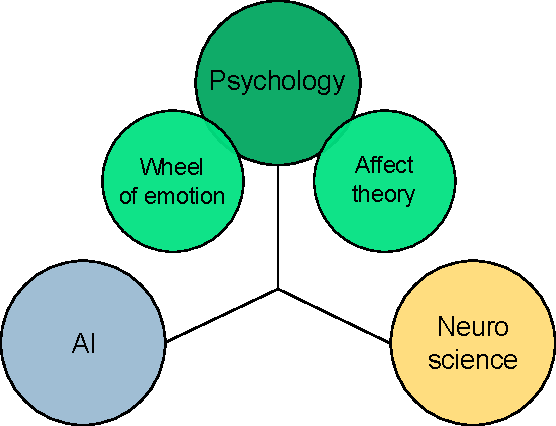
\includegraphics[height=3.5cm]{figure1_3_bases}
\end{center}
\caption{Theoretical bases of current work.}
\label{3_bases}
\end{figure}

Firstly we wanted to gain overall picture of human emotional processes. It could be understood as combination of high level processes and model that triggers processes steps. This lead us to the first base: the evolutionary psychology theory of Plutchik "Wheel of emotions" \cite{natureofemotions}. In comparison to other classifications of emotions it provides complete picture of basic and high level emotions as combination of basics and emotional processes (feedback loops). For extensive description please see Emotional Feedback Loops section~\ref{sec:feedback_loops}. We adapted feedback loops into ``Model of six'' \cite{emotionmachine} thinking levels of Marvin Minsky's cognitive architecture.

As we gained overall picture of the human emotions, we faced the lack of understanding of low level mechanism that actually triggers the affects (emotions), this lead us to neurobiological hypothesis of L\"{o}vheim: neuromodulatory base of emotions \cite{cubeofemotions}. ``Cube of emotions'' by it self based on the ``Theory of affects'' by Tomkins \cite{primer_affect_psychology, tomkins1, tomkins2, tomkins3}.

We gained proper philosophical context by means of Marvin Minsky book ``The emotion machine''. This book shades the light on really complex phenomena like: consciousness, thinking, imagination and so on. We intensively used ``Model of six'' the model of six layers of mental activities:

\begin{enumerate}
 \item Instinctive Reactions
 \item Learned Reactions
 \item Deliberative thinking 
 \item Reflective Thinking
 \item Self-Reflection
 \item Self-Conscious Reflection
\end{enumerate}

We mapped all the theories described above on Marvin Minsky's cognitive architecture described in his book "The emotion machine" \cite{emotionmachine}.

\section{Emotional Feedback Loops}
\label{sec:feedback_loops}

Robert Plutchik created the three dimensional model \cite{natureofemotions} called "Wheel of emotions", that we used to describe subjective perception of emotions. There are eight basic emotions grouped in pairs:

\begin{enumerate}
 \item  Joy - sorrow
 \item  Anger - fear
 \item  Acceptance - disgust
 \item  Surprise - expectancy
\end{enumerate}

Model presented above could be understood as the base for the subjective picture of emotions. The other indeed important for understanding the emotions aspect presented by Robert Plutchik is emotional processes or feedback loops. He introduced 8 steps process:

\begin{enumerate}
 \item{Stimulus event}
 \item{Inferred cognition}
 \item{Feeling state}
 \item{Physiological arousal}
 \item{Impulses to action}
 \item{Overt behaviour}
 \item{Effect}
\end{enumerate}

Robert Plutchik describes it as: ``Overall, emotion is a kind of homeostatic process in which behavior mediates progress toward equilibrium; I call it a behavioral homeostatic, negativefeedback system. Emotion is a chain of events made up of feedback loops. Feelings and behavior can affect cognition, just as cognition can influence feeling.'' \cite{natureofemotions}. Actions ``feeling state'' and ``physiological arousal'' are done in parallel. We interpreted this processes in four layers of Marvin Minsky's ``Model of six'' our interpretation is not direct: we combined inferred cognition with feeling state and physiological arousal in affective appraisal and neuromodulation, we selected cognitive appraisal as separate step and put it on learned reactions layer. The distinction between affective appraisal and cognitive appraisal was inspired by \cite{emotionsbraintorobot, neuromodulatory} the potential neuromodulation pathway: from spinal cord, to hypothalamus and nucleus of the solitary tract then to amygdala and septum and then to cingulate cortex and frontal cortex. So firstly every stimulus is been processed by: spinal cord, hypothalamus and nucleus of the solitary tract, then amygdala and septum, non-consciously, and then cingulate cortex and frontal cortex could impact to the whole emotion processing consciously in case of frontal cortex. Mapping of emotional feedback loops to ``Model of six'' is presented on the figure~\ref{orchestra_of_emotions}.

\begin{figure}
%\vspace{10cm}
\begin{center}
 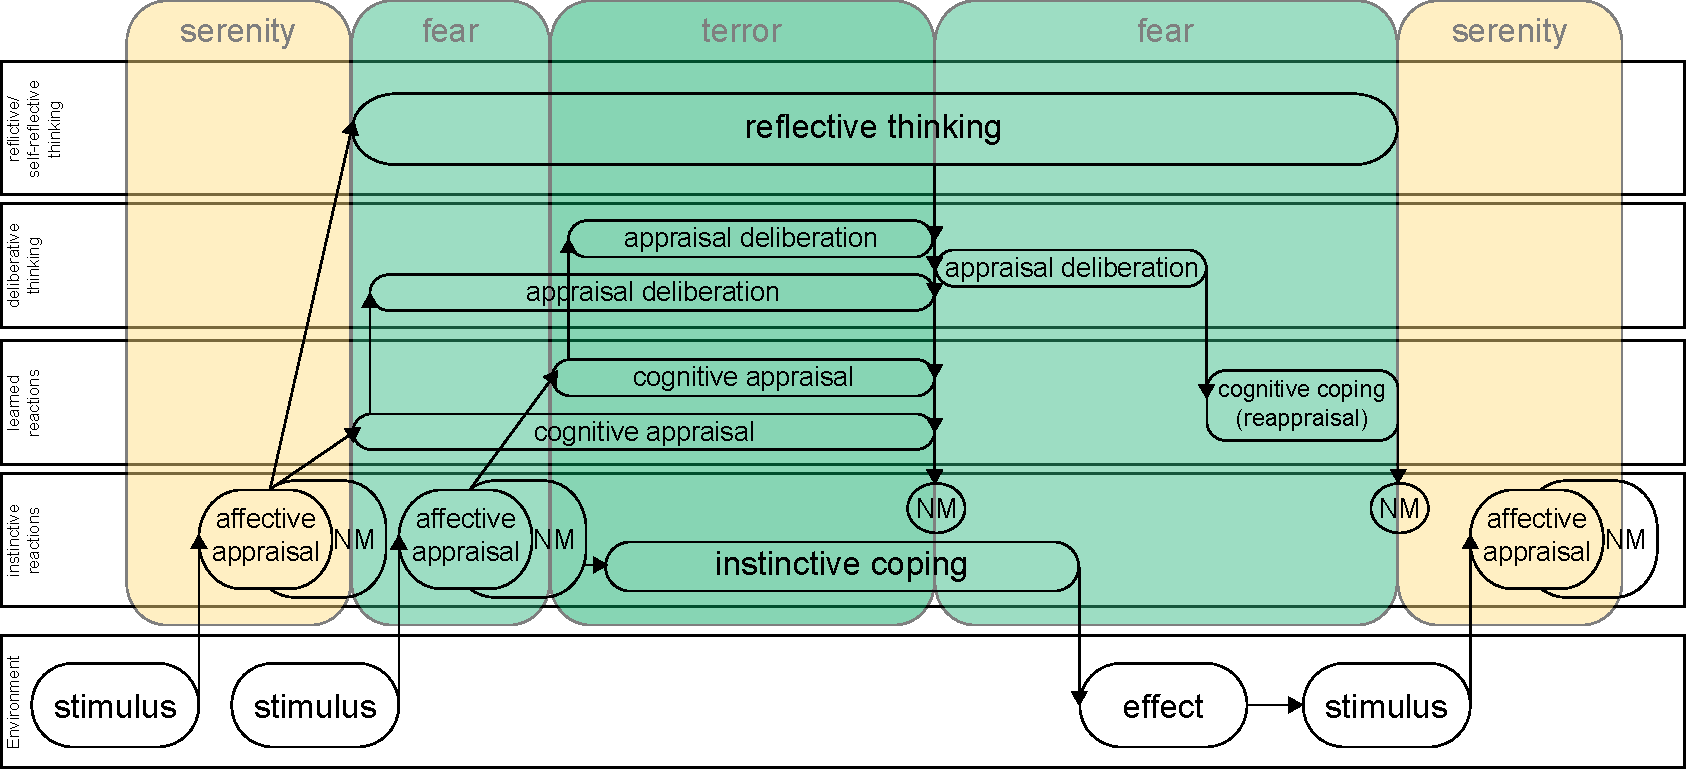
\includegraphics[height=10cm, angle=90]{figure2_orchestra_of_emotions}
\end{center}
\caption{Orchestra of emotions \label{orchestra_of_emotions}}
\end{figure}

We use five of the six layers just for the purpose of this example. Self-conscious reflections layer could influence emotions; for example evaluation of self as not progressing could cause sorrow or even depression, but it was not shown on the diagram.

We correspond instinctive reactions layer with non-conscious, innate, affective responses that mainly takes palace in: hypothalamus and amygdala, only after the frontal cortex is triggered in stimulus processing becomes conscious. This way any stimulus is being processed first unconsciously; this is shown as affective appraisal oval, and then consciously, this is shown as cognitive appraisal oval.

Using a concrete example presented on figure~\ref{orchestra_of_emotions}: first stimulus triggers affective appraisal and affective appraisal triggers neuromodulation. Neuromodulation triggers an emotional state switch from serenity to fear, depicted by yellow and green rectangle. \footnote{Emotional states are represented as rounded rectangles on the diagram.} Affective appraisal triggers cognitive appraisal and reflective thinking. \footnote{Actions like appraisals, deliberations, copings and neuromodulations are represented as ovals on the diagram, initiation or triggering are shown on diagram as arrows.} Cognitive appraisal in its turn initiates a appraisal deliberation process. Meanwhile second stimulus triggers second affective appraisal and its neuromodulation switches emotional state from fear to terror. Second affective appraisal triggers cognitive appraisal that in its turn initiates second appraisal deliberation. Then reflective thinking process estimating all activities in mind realizes that it's too emotional now and then stop all appraisal related processes and starts new coping oriented deliberation and switches emotional state via neuromodulation from terror to fear. Third appraisal deliberation selects cognitive reappraisal as coping strategy and this coping strategy is executed and switches emotional state back to serenity (via neuromodulation).
In parallel to all cognitive and reflective process the second affective appraisal initiates non-conscious instinctive coping strategy and it when applied created an effect over environment and this effect is been appraised again as stimulus.

\section{Neuromodulatory Basis of Artificial Emotions}

Hugo L\"{o}vheim in 2012 published article "A new three-dimensional model for emotions and monoamine neurotransmitters" \cite{cubeofemotions}. Axes of the model are neuromodulators (monoamines): serotonin, dopamine, noradrenaline. ``As each of these three monoamine systems probably represents a different aspect of emotion, a hypothetical three-dimensional space for possible combinations is formed. It is evolutionarily rational that the monoamine systems are mutually orthogonal as this maximizes the amount of information that can be transmitted, however, although likely, this needs to be further established empirically. It is important to note that as long as none of the monoamines transmit exactly the same information as any other (which seems unlikely), there will still be a three-dimensional space. For simplicity, in this article the monoamines axes have been depicted as mutually orthogonal.''

Vertexes are affects from Tomkins affect theory \cite{primer_affect_psychology}. ``The psychologist Silvan Tomkins devoted his life to the study of emotions and developed an elaborate and comprehensive theory of basic emotions[85–87,89]. Tomkins identified eight basic emotions, which he labeled with one word for the emotion when it was of low intensity and another word for the same emotion at a higher intensity[98,99]. Tomkins referred to basic emotions as ‘‘innate affects’’ where affect, in his theory, stands for the ‘‘strictly biological portion of emotion’’[83]. According to his theory, these are the eight basic emotions:''

\begin{enumerate}
 \item  Enjoyment/Joy
 \item  Interest/Excitement
 \item  Surprise
 \item  Anger/Rage
 \item  Disgust
 \item  Distress/Anguish
 \item  Fear/Terror
 \item  Shame/Humiliation
\end{enumerate}

Hugo L\"{o}vheim gives extended explanation of mapping of each neurotransmitter to group of emotions that he inherited from Tomkins ``Theory of affects''. We placed several quotes here form ``A new three-dimensional model for emotions and monoamine neurotransmitters'' \cite{cubeofemotions} for sake of justification of neurotransmitters choice.


\subsection{Fear/terror and anger/range}

``Both of the basic emotions, fear/terror and anger/rage, are supposedly high-dopaminergic and therefore coupled to reinforcement[9,101–104]. This seems logical when one considers the great evolutionary value of learning about those dangerous situations in which these negative basic emotions are triggered. It has been found that laboratory rats easily learn to avoid various stimuli presented simultaneously as something innately scary (such as a cat)[34]. The rewarding effect of these basic emotions might also possibly explain why certain people continue to seek so-called adrenaline rushes. 

... 

Both fear/terror and anger/rage are here further assumed to be low-serotonergic, as these emotions are triggered when the individual feels threatened or under pressure, and therefore probably has an inner feeling of weakness. Aggression has also been coupled to serotonergic deficit in many studies, supporting the placement of anger/rage on the low-serotonergic side[10,19,27,28,52,53].

...

High-noradrenergic emotions are supposedly those where the individual is active and aroused, attentive, with a high pulse [5,33,45,47,50]. The basic emotion fear/terror has been placed in the low-serotonergic, low-noradrenergic, high-dopaminergic corner of the cube. This basic emotion should not be confused with the active ‘‘fight or flight’’ reaction; instead fear/terror is considered here the ‘‘white, cold’’ fear, when the heart almost stops beating.''

\subsection{Shame/humiliation and distress/anguish}

``Distress/anguish is placed in a corner close to shame/humiliation, as the active (and hence noradrenaline-high) analogue to shame/humiliation, i.e. where noradrenaline is supposedly high and dopamine and serotonin are low. The relation between shame and depression [115–117], and anxiety and depression [118] respectively, supports the placing of these two basic emotions on the low-serotonergic side, as do the effect of SSRI antidepressants on anxiety disorders[119], and an increased serotonin transporter binding in generalized social anxiety disorder[120,121]. The association between shame and anxiety supports the decision to place these two basic emotions close to each other[122,123].''

\subsection{Interest/excitement and enjoyment/joy}

``Interest/excitement has been placed in the corner of the cube where all three monoamines are high. This basic emotion is, therefore, according to this model, active, reinforcing and coupled to a basic feeling of inner strength. One archetypal form of excitement is sexual excitement, but this basic emotion might accompany a wide range of events, perceptions or thoughts.

...

Enjoyment/joy is suggested as the low-noradrenergic analogue to interest/excitement. Another word for this basic emotion might
be contentment, and compared to the basic emotion of interest/excitement the individual experiencing enjoyment/joy is calm and relaxed.''

\subsection{Contempt/disgust}

``Disgust might, therefore, be somewhat related to satiety, in its extreme. This points towards disgust being high-serotonergic, as do the reduced ability to recognize disgusted faces found in healthy individuals after tryptophan depletion[160] and among patients with severe depression [161] or social anxiety disorder[162]. ... The relation between shame/humiliation and contempt/disgust has been described as self-contempt versus contempt for an object[86], and therefore, it seems logical that the difference between these basic emotions, according to the model, is the serotonergic state, assumed to be related to inner strength and self-confidence.

Disgust is supposedly low-dopaminergic as it is in many ways the direct opposite of reinforcement. Contempt/disgust is closely
related to repulsion and withdrawal; we usually stop eating when we feel disgust.''

\subsection{Surprise}

``Surprise has been placed in the high-serotonergic, low-dopaminergic, high-noradrenergic corner, and might thus be regarded as the non-reinforced analogue to excitement, which seems logical considering that surprise has been described as a neutral basic emotion. At the same time surprise is a highly focused, attentive state, and therefore logically high-noradrenergic. Also, according to the model, the individual experiencing surprise as compared to distress/anguish has a basic feeling of confidence and inner strength.''

L\"{o}vheim proposed monomaines based emotion regulation system: ``The monoamine-releasing upper brain stem areas – raphe nuclei, ventral tegmental area and locus ceruleus - do not, however, ultimately control our emotions. There is a growing body of evidence suggesting a crucial role for the amygdala and other limbic structures in the synthesis of information and control of behaviors and emotions [34–44]. These structures handle the processing of emotion-eliciting information and trigger certain emotions in certain situations, and are projecting towards the monoaminergic nuclei which serve to deliver the message – the emotion – to the whole brain [5,41,43]. In other words, the monoamine transmitter systems might form one final pathway for the simultaneous delivery of emotional information to large and dispersed areas of the brain.''

\section{Monoamines Neuromodulators to Computing Parameters Mapping}

Mostly low level influence of affects on brain we could call it cellular or neuronal is described above and provides fundamental base for our affective computation model. Noradrenaline, serotonin, dopamine do not have direct mapping on computational processes, for obvious reasons current computers do not have anything in common with biochemical processes in neurons. The most reasonable way we observe at the moment is to create an indirect mapping based on role of each neuromodulator involved in human emotions. In other words we draw an analogy between computational processes in computer and neurotransmission in brain and corresponded biochemical influence of neuromodulatory systems on neurons with influence of virtual neuromodulators levels on computational processes of a machine. We used several works to gain proper picture and understanding of neuromodulation and neuromodulatory systems \cite{cubeofemotions, neuromodulatory, on_role_of_emotion}. 

Especially interesting from our perspective is an article ``Emotions: from brain to robot'' \cite{emotionsbraintorobot}, where the role of dopamine, serotonin and their impact in emotional context is discussed. It could be considered as one of bases of our work in neuromodulation domain.

\subsection{Dopamine}

``In the mammalian brain, dopamine appears to play a major role in motor activation, appetitive motivation, reward processing and cellular plasticity, and might be important in emotion. Dopamine is contained in two main pathways that ascend from the midbrain to innervate many cortical regions. Dopamine neurons in the monkey have been observed to fire to predicted rewards[67,68]. Moreover, dopamine receptors are essential for the ability of prefrontal networks to hold neural representations in memory and use them to guide adaptive behavior. Therefore, dopamine plays essential roles all the way from ‘basic’ motivational systems to working memory systems essential for linking emotion, cognition and consciousness.''

According to L\"{o}vheim \cite{cubeofemotions} dopamine is associated with ``[r]eward, reinforcement, motivation''.

From computational system perspective we interpret dopamine impact like: it plays role in: reward processing thus in decision making, working memory - memory distribution and storage in computing system, motivation - decision making.

\subsection{Serotonin}

``Serotonin has been implicated in behavioral state regulation and arousal, motor pattern generation, sleep, learning and plasticity, food intake, mood and social behavior [69]. The cell bodies of serotonergic systems are found in midbrain and pontine regions in the mammalian brain and have extensive descending and ascending projections. Serotonin plays a crucial role in the modulation of aggression and in agonistic social interactions in many animals. In crustaceans, serotonin plays a specific role in social status and aggression; in primates, with the system’s expansive development and innervation of the cerebral cortex, serotonin has come to play a much broader role in cognitive and emotional regulation, particularly control of negative mood or affect.''

L\"{o}vheim associates serotonin with ``[s]elf confidence, inner strength, satisfaction''.

Thus our interpretation of influence of serotonin system looks like: decision making of the system is influenced by serotonin, confidence and satisfaction as coloring of the knowledge is impacted by serotonin too, this way serotonin should influence training of machine and storage of the information learned.

\subsection{Noradrenaline}

Hugo L\"{o}vheim \cite{cubeofemotions} emphasizes the noradrenaline role in: ``Attention, vigilance, activity''. Then he describes the role of noradrenaline: ``while noradrenaline has been coupled to the fight or flight response and to stress and anxiety, and appears to represent an axis of activation, vigilance and attention''. Robert D. Hunt describes role of noradrenaline (NE) and its impact on cognitive functions \cite{norepinephrine} : ``NE has an emerging role in several essential processes: (1) maintaining and increasing overall arousal, (2) contributing to affect regulation related to excitability and response to danger or opportunity, and (3) contributing to memory storage and retrieval, especially affect-related or emotionally intense events. While NE has a critical role in emergency response, it also assists in maintaining basal or tonic alertness. At a quieter moment, reading a book, studying at night, the effort to remain alert and stay on task partially mediated by NE.[3]''

The noradrenaline or it is better to call it virtual noradrenaline could influence modern computational system like this: the attention and concentration could impact computing power and memory distribution between processes and threads (here we mean the operating system processes and memory available for operating system), alertness also impact distribution of computing power and memory of the system. The decision making is influenced by alertness effect of noradrenaline reducing number of options in the observation, and possibly making system use more risky choices. 

\subsection{Computational system parameters}

We introduced several computing system parameters in previous three sections. According to their nature we split them in two groups: most obvious generic parameters of computing system that includes: computing power, memory distribution, learning and storage; decision making is massively impacted by affects(emotions) that made us use second special group including: confidence, satisfaction, motivation, number of options to process, tendency to use risky choices. The computing power and memory distribution are closely related parameters that heavily influence resources of a system used for current activity (cognitive process). The storage is influenced by learning forming the information to store during the training. The decision making group represents parameters and coloring (tagging, flagging) of the trained information exploited during making the decision processes. The confidence impact on decision making is one of the most obvious and important, even the selection of the information is done taking in account how system is confident in this information. The satisfaction is one of most important flags involved in reward system \footnote{Reward system Wikipedia page: \url{http://en.wikipedia.org/wiki/Reward_system}} usually making system to select most satisfactory/pleasureful actions (approaches). The motivation \footnote{Motivation Wikipedia page: \url{http://en.wikipedia.org/wiki/Motivation}} drives system to make most desirable selections and heavily influences selections of further activities. The number of options to process and inclination to risky actions are liked to noradrenaline stressful situation alertness, both of them makes system do quick decisions with tendency to risk.

Our understanding of the role of neuromodulators  is represented in following mapping of neuromodulators to computing system parameters, the figure~\ref{cube_of_parameters}.

\begin{figure}
%\vspace{5cm}
\begin{center}
 \includegraphics[height=8cm]{figure3_cube_of_parameters}
\end{center}
\caption{Cube of parameters}
\label{cube_of_parameters}
\end{figure}

\subsection{Computing system parameters}

\begin{enumerate}
 \item  Generic:
 \begin{enumerate}
  \item  Computing power: noradrenaline
  \item  Memory distribution (attention): noradrenaline
  \item  Learning: serotonin, dopamine
  \item  Storage: serotonin, dopamine
 \end{enumerate}
 \item  Decision making/reward processing:
 \begin{enumerate}
  \item  Confidence: serotonin
  \item  Satisfaction: serotonin
  \item  Motivation, wanting: dopamine
  \item  Number of options to process: noradrenaline
  \item  Risky choices inclination: noradrenaline
 \end{enumerate}
\end{enumerate}

\subsubsection{Generic}

\emph{Computing power}: distribution and priority of parallel process or load balancing, is impacted by noradrenaline: the higher the level of noradrenaline is the more computing power must be concentrated on current activity (neuromodulator regulating attention).

\emph{Working memory(short term)} distribution and concentration is impacted by noradrenaline (attention).

\emph{Learning} is impacted by serotonin and dopamine: dopamine plays major role in activation of previously remembered patterns and serotonin in pattern generation.

\emph{Storage} management (long term memory) is impacted by both by serotonin and dopamine, higher concentrations of both neuromodulators makes system better remember stimulus. In general, strong emotions generate more persistent memories.

\subsubsection{Decision making}

This decision making is done mainly in deliberation and learned reaction layers of model of six.
Parameters: confidence, satisfaction, risky are used to highlight actions stored(remembered).

\emph{Confidence and satisfaction} of the system is influenced by serotonin.

System is more \emph{motivated} under the influence of dopamine.

System tends to choose \emph{risky} actions under the influence of noradrenaline.

Noradrenaline makes system consider a smaller \emph{number of options} in width and depth to be processed during deliberation.

This mapping is exhaustively described in ``Computational emotional thinking and virtual neurotransmitters'' \cite{computational_emotional_thinking}. It could be used as a low level model of emotional processes and could be used as a basic framework for the emotion enabled systems \cite{whatdoesitmeanforcomputer}.

\section{Cognitive Architecture Analysis}

To understand the current scientific state of affairs, existing models and implementations in actual code, and to find proper a base for our implementation we used the most traditional way: run a comparative analysis. It worth to mention that we don't want to limit ourselves with the emotion-oriented architectures; we rather want to get a wide view on the current situation in the domain. We analyzed 27 cognitive architectures.

Criteria are organized in three groups: emotional group depicts our interest in emotions implementation in cognitive architecture \cite{computationalmodelsemotionscognition}, thinking levels are the compatibility with Marvin Minsky's "The emotion machine", AI components group is used to gain understanding of width of coverage of AI domains by cognitive architecture. We used two additional criteria that seem to play important role and were not in previous groups: parallel processing, self-emergent/self-organized. Exhaustive analysis is available on-line \footnote{Exhaustive analysis address: \url{https://github.com/development-team/2/blob/master/doc/analysis/cognitive_architecture.md}}.

We used primitive Boolean approach to measure if component or emotional criteria are in specific cognitive architecture. Cumulative table is available on-line\footnote{Cumulative table address: \url{https://github.com/development-team/2/blob/master/doc/analysis/cognitive_architecture.md}}, it contains simple summary of the Boolean criteria.

According to our brief overview of the list of architectures most interesting are: ASMO, CLARION, DUAL, \emph{H-CogAff}, LIDA, \emph{Psi-Theory}, Soar, \emph{Society of mind} (*), WASABI, EMA, Hikonen, Shanahan.
H-CogAff is more of philosophical framework to build the cognitive architecture, or a meta-architecture that has the most significant potential to be the most advanced at the moment and the least limited. Homeostatic principle of Psi-Theory seems to be ubiquitous in the psychological basis of emotions \cite{natureofemotions}. Society of mind needs further analysis and possible update of our criteria.

\section{Possible implementation and validation}

The emotional neuromodulation is connected to reward system \cite{neuromodulatory, emotionsbraintorobot, primer_affect_psychology, appraisal_considered_as_a_process, computationalmodelsemotion, dont_worry_be_happy, roleOfReinforcement} first of all we supposed that most appropriate would be the implementation of this affective computation model as realistic neural network (like NEST \footnote{NEST project Wikipedia page: \url{https://en.wikipedia.org/wiki/NEST_(software)}}), placed in the life threatening situation. Classical example is zapping rat (brain) \footnote{\url{http://www.nature.com/news/flashes-of-light-show-how-memories-are-made-1.15330}}. Potential disadvantage of this reward oriented implementation and thus validation is that reinforcement learning  \footnote{Reinforcement learning Wikipedia page: \url{http://en.wikipedia.org/wiki/Reinforcement_learning}} could be used in the same life threatening situation with similar effect. The attention is one most important phenomena that is heavily influenced by affects \cite{neuromodulatory, on_role_of_emotion, emotionsbraintorobot}, neuromodulation of noradrenaline. Taking in account both effects on reward system and attention we plan to implement neuromodulation mechanism of three monoamines over realistic neural network \footnote{The list of realistic NNs: \url{http://home.earthlink.net/~perlewitz/sftwr.html}}. In the life threatening situation behavioral difference between emotional and non-emotional neural network should be obvious enough to indicate the advantages/disadvantages of emotional reactions. Other way to validate the emotional framework could be comparative test of non-emotional reinforcement learning with emotional reinforcement learning. Neuromodulation based affective computation model could contribute to it at least by distribution of resources (attention) and communicating to other agents (is not discussed in this paper) \cite{on_role_of_emotion}. Thus implementing described above model we should be able to notice behavioral and resources delta impacted by neuromodulation and thus affects.

\section{Conclusion}

We presented computational model of the affective influence on computational processes we used following starting points: Robert Plutchick "Wheel of emotions" \cite{natureofemotions, senticcomputing} as high level picture of emotions, Tomkins ``Theory of affects'' \cite{primer_affect_psychology} as framework of affects/emotions, Hugo L\"{o}vheim "Cube of emotions" \cite{cubeofemotions} as neurophysiological mechanism of emotions and Marvin Minsky "The emotion machine" \cite{emotionmachine} as cognitive architecture as implementation environment for all mechanisms listed above.

This works is simplification of the several set of processes of the brain linked to affects. It does not take in account influence of tightly coupled endocrine system, digestion, heart rate and other biological processed that are influenced or influence affective state of humans, even the role of several brain structures involved in the affects processing is only implied. This simplification is based on main assumption made in article of L\"{o}vheim: the emotional regulation could be expressed in the three-dimensional model that uses monoamines relative levels as axes. 

This model does not take in account influence of opioids \cite{emotionsbraintorobot} or acetylcholine \cite{roleOfReinforcement} still we consider it as useful base for further extension for an appraisal computation that should involve modeling of brain structures and their interconnections and influences involved in the monoamine system of the brain.   

Using the role of each of monoamine neuromodulators: dopamine, serotonin, noradrenaline, in human emotions processing we proposed mapping of virtual neuromodulators on computational processes of modern computers. This mapping is represented on figure~\ref{cube_of_parameters}. We used two groups of parameters: most obvious and simple generic: computing power, computing system memory distribution, learning, computing system storage distribution; decision making group is created taking in account heavy impact of the affects(emotions) on decision making and emotional coloring that influences the decision making: confidence, motivation, number of options to process, risky choices inclination.

One of the possible implementations could be emotion enabled reinforcement learning. On the other hand the realistic implementation of brain limbic, cortical subsystems and other structures according to Damasio \cite{emotionInPerspectiveOfIntegratedNervousSystem}: ``(a) the prefrontal cortices, especially those in the ventral and medial sectors and, more broadly, in the orbital sector; (b) it also includes the somatosensory cortices, by which I refer not just to SI in the rolandic region but also to SII and to insular cortices; (c) monoamine nuclei in the brain stem; (d) periacqueductal gray; and (e) other nuclei both in the brain stem and spinal cord involved in both afferent and efferent signaling relative to viscera and internal milieu'' could provide much more interesting implementation and validation results. 

\section{Acknowledgment}

Tero Keski-Valkama (MSc) for his constant support and review of our work and hypotheses.
